%%%%%%%%%%%%%%%%%%%%%%%%%%%%%%%%%%%%%%%%%%%%%%%%%%%%%%%%%%%%%%
% NUbots' TDP 2017
%
% Date: 24.11.2016
%
%
\documentclass{llncs}
%
\usepackage{graphicx}
\usepackage[colorinlistoftodos]{todonotes}
\usepackage{verbatim}
%
\begin{document}
%

\frontmatter          % for the preliminaries
%
\pagestyle{headings}  % switches on printing of running heads
\addtocmark{The NUbots Qualification material for RoboCup 2018} % additional mark in the TOC
%
%
\mainmatter              % start of the contributions
%
\title{The NUbots Team Description Paper 2018}
%
\titlerunning{The NUbots Team Description for 2018}  % abbreviated title (for running head)
%                                     also used for the TOC unless
%                                     \toctitle is used

\author{Matthew Amos
        \and Alex Biddulph
    %   \and Elliot Catt
        \and Stephan Chalup
        \and Luke Farrawell
	%	\and Jake Fountain
        \and Daniel Ginn
        \and Trent Houliston
    %   \and Tony Jackson
    %   \and Robert King
    %   \and Zachary Mason-Roach
		\and Alexandre Mendes
    %   \and Mitchell Metcalfe
        \and Josephus Paye
	%	\and Anita Sugo
        \and Peter Turner
    %   \and Josiah Walker
        \and Taylor~Young
        }
       
%
\authorrunning{Amos et al.}   % abbreviated author list (for running head)
%
%%%% modified list of auth for the TOC (add the affiliations)
\tocauthor{
M. Amos,
A. Biddulph,
S. Chalup,
L. Farrawell
D. Ginn,
T. Houliston,
A. Mendes,
J. Paye,
P. Turner,
T. Young
}

%
\institute{Newcastle Robotics Laboratory\\ School of Electrical Engineering and Computing\\
Faculty of Engineering and Built Environment\\
The University of Newcastle, Callaghan 2308, Australia\\
Contact: \email{stephan.chalup@newcastle.edu.au}\\
Homepage: \texttt{http://robots.newcastle.edu.au}}
%

\maketitle              % typeset the title of the contribution


\begin{abstract}
The NUbots are the RoboCup team of the The University of Newcastle in Australia. In 2018 they play for the first time in the Teen-size Humanoid League using their self-printed robots based on the Igus-Nimbro design. In previous years the NUbots participated in the Standard Platform League (2002-2011) and the Kid-size Humanoid League (2012-2016). Over the past two years the NUbots have developed the NUClear software framework which is a modern software architecture specifically developed for robot projects. The NUbots' research addresses applications of machine learning, software engineering and computer vision. Their current research focus is Deep Learning. This paper provides an overview of the NUbots team, its software system and robot platform. 
\end{abstract}

%
\section{Introduction}
For 15 years the Newcastle Robotics Laboratory has been hosting the NUbot robot soccer team as its central project. The NUbots previously competed at RoboCup in the Four-Legged League, the Standard Platform League and until 2017 in the Kid-Size Humanoid League. They now step-up to the Teen-size Humanoid League where they are a newcomer. The goal of the 2018 NUbot team is to demonstrate exciting state-of-the-art robot soccer skills using their modified Igus-Nimbro~\cite{allgeuer2016igus} based robot platform---the NUgus.  

%The NUbots' mission is to achieve high quality research results while contributing to a responsible development and application of robotics that can support humans not only for routine, challenging, or dangerous tasks, but also to improve quality of life through personal assistance, companionship and coaching. Some of the lab's research projects therefore emphasise anthropocentric and biocybernetic aspects in robotics~\cite{ChalupOstwald2009,WalkerChalup2015,HongEtAl2014,WongEtAl2012,WongEtAl2013}. 
The following sections describe research and history of the NUbot team. Some of the material, such as the history and previous research, was already covered by~\cite{AmosEtAl2017}.


\section{Scientific Aspects of the NUbot Humanoid Robot System and  Research Interests of the Lab and Team}
 
The scientific aspects of the current NUbot system involve deep learning on robots, software engineering for robotics and AI, as well as various aspects of computer vision, localisation, human-robot interaction  and machine learning.

\subsection{Current Research Projects in the Newcastle Robotics Lab}
The following paragraphs briefly describe some of the NUbots' current projects, where more details on the NUbots research in the past 15 years can be found, e.g., in~\cite{AmosEtAl2017} and the relevant webpages, e.g., at
\texttt{www.robots.newcastle.edu.au}.\\

\noindent\textbf{Deep Learning in Robotics:} 
Deep learning has become a central topic of research in the lab. Several PhD and undergraduate projects involve deep learning. Tensorflow and Caffe have been integrated into the NUbots' system and trialled for the tasks of face and pedestrian detection. On the topic of deep learning there are two recent publications. They address the topics of scene sentiment analysis where several deep networks were combined into a larger system \cite{AbbasChalup2017}, and the use of synthetic data generated by computer graphics techniques for training deep nets on object detection tasks~\cite{JabbarEtAl2017}.\\

\noindent\textbf{Software Engineering for Robotics:} Much work has been focused on the underlying software architecture and external utilities to enable flexibility and extensibility for future research \cite{Kulk2011c,HoulistonEtAl2016}. Projects undertaken include improving the configurability of the software system via real-time configuration updates, development of a web-based online visualisation and debugging utility \cite{AnnableEtAl2014} and the application of software architectural principles to create a multi-threaded event-based system with almost no run-time overhead. Some of this work is still in progress.\\ %by new undergraduate and postgraduate students who are associated with the lab.\\ %\cite{BilleEtAl2016}.\\

\noindent\textbf{Manifold Learning and Alignment:} In several past projects we investigated non-linear dimensionality reduction
methods in order to achieve more accurate processing of high-dimensional motion, visual and acoustic data. %\cite{WongEtAl2012}. 
Manifold alignment is part of an on-going PhD project using simulated data~\cite{AzizEtAl2015}. Another new research topic is the use of persistent homology for data analysis \cite{PaulChalup2017}.\\

\noindent\textbf{Robot Vision:}  Several topics have been investigated including object recognition, horizon determination, edge detection, model fitting and colour classification using ellipse fitting, convex optimisation and kernel machines. Recent work has resulted in a fully-autonomous method of colour look-up table adaptation for changing lighting conditions, allowing us to overcome one of the major limitations of the colour look-up table system. Recent publications are available e.g. %from~\cite{budden2012colour,budden2012ball,henderson_2007,nicklin_2007,NUBOT2006,QuinlanEtAlNIPS2003,Henderson2008,HoulistonEtAl2015,MetcalfeEtAl2016}.
from~\cite{HoulistonEtAl2015,MetcalfeEtAl2016}.\\

\noindent\textbf{Localisation:}  
Motivated reinforcement learning was employed to optimise head movement behaviour, allowing a robot to learn to choose landmarks to localise efficiently during a soccer game~\cite{FountainEtAl2014}. Visual SLAM point-clouds based on Semidirect Visual Odometry (SVO)~\cite{forster2017svo} are also being enhanced with semantically labelled objects which will allow for merging with map priors of the soccer field.




%\subsection{Summary of previous relevant achievements in research and development as well as publications}
%Machine learning on robots has been of central interest for the NUbots for a long time \cite{ChalupEtAlSMC2007}.In recent years the NUbots have engaged in a variety of research projects some examples include machine learning on robots \cite{ChalupEtAlSMC2007,FountainEtAl2014,AzizEtAl2015}, computer vision \cite{MetcalfeEtAl2016}, robot walk \cite{Kulk2011c,Kulk2010}, and anthropocentric and biocybernetic computing~\cite{WalkerChalup2015,HongEtAl2014,WongEtAl2013}.

%\noindent\textbf{Localisation and Kalman Filters:} Research on the topic of localisation focused on Bayesian approaches to robot localisation including Multi-modal Unscented Kalman Filters and particle filter based methods. Since the Robocup Kidsize environment is becoming more complex to localise in, we are investigating efficient methods to integrate often non-ideal information from vision. One of the team members is working on the use of information about the surroundings of the playing field for localisation purposes. We are also interested in modifications for localisation which incorporate information from multiple agents, and utilise rich motor and kinematics data for odometry and sensor fusion. Current work in  improving sensor fusion includes neural processing to determine foot-ground contact for odometry, and the implementation of body position and velocity tracking. These improvements allow us to efficiently implement a vestibulo-occular head reflex to reduce image blur when moving.
%Furthermore we are also interested in the use of machine learning to
%improve the models used by localisation. For information about our current approach see
%\cite{robocup_2009}.

%\noindent\textbf{Development of the Robot Bear:} In a collaborative effort with the company Tribotix and colleagues in design, a bear-like robot (called Hykim) was developed~\cite{ChalupEtAl2006}. It has a modular open platform using Dynamixel servos.

%\noindent\textbf{Biped Robot Locomotion:} The improvement of walking speed and stability has been investigated by the NUbots for several years and on different platforms: On the AIBO robot we achieved one of the fastest walks at that time by walk parameter evolution \cite{QuinlanEtAlACRA2003,ChalupEtAlSMC2007}. On the Nao robot we improved existing walk engines by modifying the joint stiffnesses, or controller gains, \cite{Kulk2008,Kulk2010} and by applying optimisation. % Kulk2010a
%The stiffnesses were selected through an iterative process to maximise the cost of transport. We investigated the application of Support Vector Machines and Neural Networks to proprioception data for sensing perturbations during pseudo quiet stance. Walk improvements have been primarily done via optimisation techniques \cite{Kulk2011a},  %,Kulk2011b
%with recent improvements to our framework for online optimisation of bipedal humanoid locomotion.
%The use of spiking neural networks has been trialled in simulation~\cite{WiklendtChalup2008}. Prior to RoboCup 2012 the walk engine developed by the leading SPL team BHuman~\cite{BHumanWalk2010} was ported to the DARwIn-OP platform, and a variety of optimisation techniques were developed and successfully applied to improve walking speed and stability of the DARwIn-OP walk. Recent work conducted by two of our students has focused on improving the modularity of the walk engine to improve portability and enable new research. %\cite{budden2013probabilistic}. Multi-agent walk optimisation is being developed for this year's competition.

%\noindent\textbf{Reinforcement Learning, Affective Computing and Robot Emotions:} We investigate the feasibility of reinforcement learning or neurodynamic programming for applications such as motor control and music composition. Concepts for affective computing are developed in multidisciplinary projects in collaboration with the areas of architecture and cognitive science. The concept of emotion is important for selective memory formation and action weighting and continues to gain importance in the robotics community, including within robotic soccer~\cite{HongEtAl2014,FountainEtAl2014,ChalupOstwald2009,WalkerChalup2015,WongEtAl2012,WongEtAl2013}.

%\noindent\textbf{Gaze analysis and head movement behavioural learning:} We investigated methods for human and robot pedestrian gaze analysis in~\cite{JalalianEtAl_CAADRIA2011,WongEtAl2012} as well as space perception, way finding and the detection and analysis of salient regions~\cite{BhatiaEtAl2013,BhatiaChalupOstwald2013}. More recently 


\subsection{Background and Research Interests of the NUbots Team Members}

\begin{itemize}
\item \emph{Matthew Amos} is a fifth year undergraduate student studying a combined degree in Computer Science and Computer Engineering. He is interested in computer vision and machine learning.

\item \emph{Alex Biddulph} is studying for a Doctorate of Philosophy in Computer Engineering. Alex has undergraduate degrees in Computer Engineering and Computer Science with Honours in Computer Engineering. The focus of Alex's studies will revolve around the symbiotic relationship between hardware and algorithms, with a focus on computer vision.

\item \emph{Associate Professor Stephan Chalup} is the head of the Newcastle Robotics Lab. His current research focuses on deep learning, neural information processing systems and topological data analysis.

\item \emph{Luke Farrawell} is a recent Software Engineering (Honours) graduate and research collaborator. His interests include robotics, computer graphics and virtual reality. He contributes to NUsight; the real-time web based debugging environment.

%\item \emph{Jake Fountain} is studying for a Doctorate of Philosophy in Computer Science. Jake has undergraduate degrees in mathematics and science, majoring in physics, with Honours in Computer Science~\cite{FountainChalup2015}. His main interests lie in virtual reality and robotics.

\item \emph{Daniel Ginn} is pursuing a PhD in Computer Science with focus on questions of localisation and mapping using robotic platforms in the context of RoboCup. 2017 was the first time he joined the NUbots competition team.

\item \emph{Trent Houliston} is completing his PhD in software engineering focusing on software architecture for robotics and real-time computer vision. He has been a part of NUbots since 2013 and was NUbots team leader in 2016 and 2017.

%\item \emph{Anita Sugo} is a fourth year undergraduate student studying a degrees in mathematics and science, with a major in physics. She is interested in the mathematics used in robotics and is currently working on computer vision.

%\item \emph{Mitchell Metcalfe} has undergraduate degrees in mathematics and computer science, with Honours in Computer Science. He contributes to the NUbots' localisation, and motion planning systems, and has interests in computer vision and machine learning.

%\item \emph{Elliot Catt} is a final year undergraduate student studying a Bachelor of mathematics degree. His interests include number theory,  machine learning and intelligent agents \cite{CattCoonsVelich}. He is currently working on a sound based localisation project and behaviour.



%\item \emph{Tony Jackson} is a fifth year undergraduate student studying a combined degree in Computer Science and Computer Engineering. He has recently joined the NUbots team and has been contributing towards the walk engine of the robot. 

%\item \emph{Zachary Mason-Roach} is a final year undergraduate student studying a combined Bachelor degree in Computer Science and Computer Engineering (Honours). He is presently contributing to the NUbots walk engine and designing balance and push-recovery methods for humanoid robotics.  His dominant interests comprise of machine learning and robotic awareness, computer vision and mathematical applications to artificial intelligence.



%\item \emph{Dr. Robert King} is a lecturer in statistics. He has been RoboCup world champion with the NUbots in 2006 and with the NUManoids in 2008. 

\item \emph{Dr. Alexandre Mendes} is deputy head of the Newcastle Robotics Lab. He is a Senior Lecturer in Computing and Information Technology. He joined the group in September 2011 and his research areas are evolutionary algorithms and optimisation.

\item \emph{Josephus Paye} is a second year undergraduate student studying Computer Science, with a major in Computer Systems and Robotics. He contributes to NUsight, the web-based debugging environment.

\item \emph{Peter Turner} is technical staff in the School of Electrical Engineering and Computer Science. Peter provides hardware support and assists the team with physical robot design upgrades. %an expert on robot hardware and electronics and familiar with the DARwIn-OP.

\item \emph{Taylor Young} is a third year undergraduate student studying Electrical Engineering. He contributes the hardware based aspects, the design and manufacturing of the robots.

%\item \emph{Josiah Walker} is about to complete his PhD in Machine Learning where he worked on improved similarity search for large data sets. He was NUbot team leader for several years.
\end{itemize}
The current NUbot team acknowledges the input of team members of previous years and other colleagues from the Newcastle Robotics Lab. Details are linked to 
\texttt{www.robots.newcastle.edu.au}.

\subsection{Related Research Concentrations}
The \emph{Interdisciplinary Machine Learning Research Group (IMLRG)} investigates different aspects of machine learning and data mining in theory, experiments and applications. The IMLRG's research areas include: Dimensionality reduction, vision processing, robotics control and learning,  evolutionary computation, optimisation, reinforcement learning, kernel methods, and deep learning. %Links to publications can be found at the NUbots' webpage
%\begin{center}
%\texttt{http://robots.newcastle.edu.au/}
%\end{center}

\section{History of the NUbots and Prior Performance in RoboCup Competitions \cite{AmosEtAl2017}}
The NUbots team, from the University of Newcastle, Australia, competed in the Four-Legged-League from 2002-2007 using Sony AIBO ERS-210 and ERS-7 robots. The NUbots participated for the first time at RoboCup 2002 in Fukuoka in the Sony Four-Legged League (3rd place). At RoboCup 2006 in Bremen, Germany, the NUbots won the title. %Scenes from the final game are available at

From 2008 to 2011 they used the Aldebaran Nao within the Standard Platform League. They achieved a first place in 2008 as part of the NUManoid team in Suzhou, China.

The NUbots joined the Kidsize Humanoid League in 2012 with the DARwIn-OP robots, and ported their SPL codebase to the new platform. The NUbots retained a robust and fast vision and localisation system from the SPL, and ported the B-human NAO walk to the DARwIn-OP for 2012-2013. From 2014-2016 the NUbots redeveloped their software system based on the NUClear software architecture~\cite{HoulistonEtAl2015}. For the Darwins they made small modifications of the head, feet and cameras. 2017 was the first year where an Igus platform based robot was added to the NUbot kidsize team that then comprise a mixed team of DARwIn and Igus-Nimbro based robots.  Due to the league's hight restrictions the top of the Igus-Nimbro robot's skull had to be cut off. In 2017 the NUbots reached the quaterfinals in the Kidsize Humanoid League. After the competition all DARwIn-OP robots of the team retired. In 2018 the NUbots compete in the teen-size humanoid league using their NUgus robots that are based on the Igus-Nimbro design~\cite{allgeuer2016igus}.




%\pagebreak
\section{Software and Hardware Overview}
The NUbots team's software source is available from \cite{nubotsGit} and is covered under the GPL. This code includes associated toolkits for building and deploying the software. Our software is designed to work on multiple robotic platforms, and all of the individual modules have been designed to be easily used in other systems. The flexibility of our approach has been demonstrated in a deployment of the NUbots vision system on a marine platform\footnote{http://www.newcastle.edu.au/about-uon/governance-and-leadership/faculties-and-schools/faculty-of-engineering-and-built-environment/maritime-robotx-challenge-team/about-us}. The NUbots code-base is currently being ported to a larger humanoid platform, the Igus. Significant work has gone in to ensuring that the codebase and associated dependencies can be easily cross-compiled on to both 32-bit and 64-bit platforms, allowing for our codebase to be easily ported between different architectures. Further work has been put into extending architecture support to arm-based platforms.% \cite{renton2014robotx}. % The sensors and actuators are accessed using a standard format, regardless of the robot running the software~\cite{Kulk2011c}.

Following development of a new software system in 2014-2017, the NUbots are now focusing on the RoboCup Teen-size League. Their research aims include efficient vision processing; improved localisation; generic ball detection; and improving the walk engine. The NUClear based NUbot software is designed to allow new teams and team members to easily understand and innovate on existing code, and is made freely available to encourage research and innovation.


\section{Enhancements of the NUbots’ hardware and software compared to the previous year}
The NUbots team have built a team of teen sized robots, based of the Igus-Nimbro, making significant changes in the design of the platform. Some of these changes aid in an alternative manufacturing process used. A carbon fiber embedded nylon with continuous carbon fiber reinforcing is used as the main structural material in the manufacturing. Designed in a CAD program and 3D printed allowing for easy design modifications. Within this larger platform better computing power can be taken advantage of, with a Intel NUC7i7BNH being a major improvement over the Darwin-OP fit-PC2i. An upgraded vision system consisting of two Point Grey Flea3 USB3Vision cameras with large field of view equidistant spherical lenses is used. A new deep learning vision algorithm has been developed. An improved cooling solution is also being implemented to ensure that the CPU and servos remain cool.

\subsection{Details on software and hardware used from other teams}

\subsubsection{Acknowledgement of use of code for the walk engine}
The NUbots DARwIn-OP robots used a walk engine based on the 2013 Team Darwin code release. We acknowledge the source of this code. The NUbots have ported this code to C++ and restructured the logic, making numerous structural and technical changes. The current code for the NUgus robot walk is a further modification and extension of the code  that the NUbots used on their Darwins in previous years.

\subsubsection{Acknowledgement of other software used from other teams}
The NUbots NUgus robots are based on the 2016 Team Nimbro design files. We acknowledge the source of this design. The NUbots have have made modifications to the design to account for a different printing process and to improve the usability of the design. The modified design files are released under the original license~\cite{nubotsHardwareGit}.

\subsubsection{The NUbot team’s own contributions}
The NUbots vision system now utilises an efficient and intelligent image subsampling algorithm. This subsampling technique allows for fast, efficient, and accurate deep learning to be performed on high resolution images at frame rates in excess of 100 frames per second. The implemented algorithm provides guarantees over the number of sampled pixels within objects of certain sizes, allowing the user full control over the trade-off between the algorithms run time and accuracy.

The improved cooling system places extra fans and vents at strategic points around the robot to increase airflow in and around the CPU and servos of the robot.





%This year marks a major change in the software architecture of the NUBots, with improved software modularity coming from a cutting edge event based message passing system. The NUBots' architecture now has strong parallels with ROS (although without the associated overheads) and interoperability with ROS modules is planned. The NUBots software is designed to allow new teams and team members to easily understand and innovate on existing code. We plan to provide a full code release post RoboCup 2014.

%The software is broken into a number of modules. The primary modules are: vision, localisation, behaviour, and motion. An overview of our software structure can be seen in Figure~\ref{fig:platform}. The research areas applied to each of these modules are described in the research section.

%\begin{figure}[bht!]
%\begin{center}
%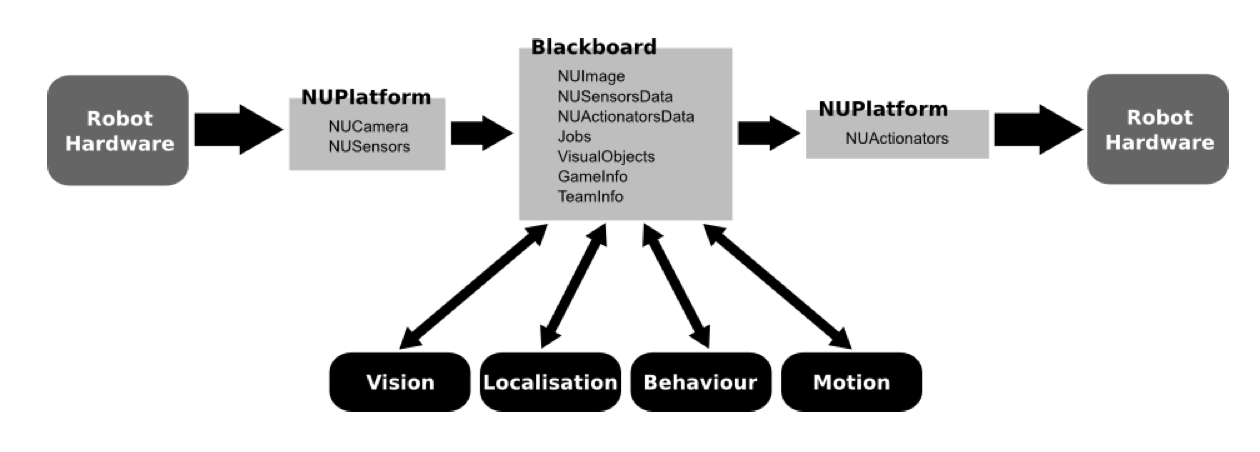
\includegraphics[width=1.0\textwidth]{Platform.png}
%\caption{An overview of the software framework, and the transfer of information between the hardware and software modules via the blackboard~\cite{Kulk2011c}.}
%\label{fig:platform}
%\end{center}
%\end{figure}

%The NUbots use seven DARwIn-OP robots with small modifications such as foot sensors and a new head. The NUbots also purchased an Igus Humanoid OP robot recently and will use it in the competition in 2017.
%The team has seven of these robots that are of the standard design with the exception of a slightly reduced foot size. %The team also hopes to field modified DARwIn-OP robots consisting of a full HD camera, an ODroid-XU computer and an updated motor communications board as a part of a student project. %Aditional minor structural modifications as well as a replacement of the main processor are planned after RoboCup 2013.

%\begin{figure}
%\begin{center}
%\scalebox{0.26}{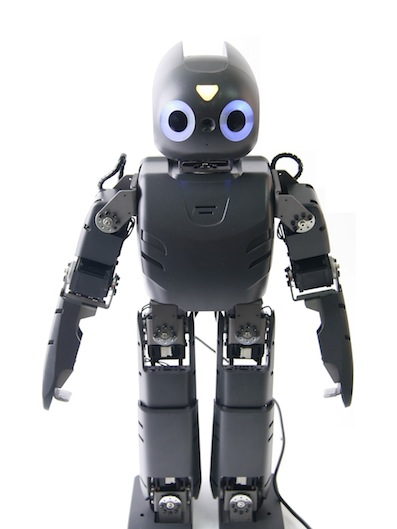
\includegraphics{darwin.png}}
%\caption{The DARWIN-OP Robot.}
%\label{fig:darwin}
%\end{center}
%\end{figure}

%\subsection{Hardware Enhancements since RoboCup 2014-2016}
%At RoboCup 2014 we trialed rapid prototyping for a new head design for the Darwin-OP robots to fit upgraded Logitech C920 cameras. In 2016 the heads went through a second prototyping phase to accommodate the Creative Labs Live! Cam Chat HD camera. %Since this time we have been improving designs and readying for an open source release once remaining issues are resolved. We field these otherwise standard Darwin-OP robots under the name NU-Darwin.

%We have been partnering with Kontron Australia to develop more powerful embedded PC boards in order to upgrade our capabilities and deploy new robotics platforms. This upgrade will see higher quality accelerometers and gyroscopes and more hardware communications channels added to the robots, as well as an upgrade to a quad-core Celeron platform with access to OpenCL.

%At the 2015 competition, soccer studs were added to the feet to allow a more stable walk. These have been iteratively refined, and during the 2016 competition it was shown that the stud design improves walk stability for other Darwin teams using different walk engines.

%In 2016, a taller Igus Humanoid OP robot was acquired. The Igus has been modified to use stereo cameras with radial lenses, which provide increased peripheral vision, and improved accuracy in the central focal region of the image.

%For 2017, the Igus Humanoid OP robot will be ready to make its competition debut. In addition, the Darwins will have an improved walk engine, with better balance and speed,  and a better localisation algorithm.

%Since RoboCup 2013, improvements have been made in the area of software architecture and hardware. As the league moves to more realistic game conditions, we are trialling a hardware control platform composed of the following:

%In response to the increase in field size, the Logitech C905 is being replaced with a Logitech C920. The new camera will provide a 1080p image, allowing the robots to detect and classify objects at greater distances.

%The Main Controller (CompuLab fit-PC2i) is being replaced by an ODroid-XU to provide the extra processing power that is required for processing the images from the Logitech C920.

%A prototype hardware replacement for the ROBOTIS CM730 Sub Controller, named the TAJ3850, is
%being developed as part of a Computer Engineering Third Year Project. The TAJ3850 provides power to all system components, a battery monitoring system featuring a low-voltage alarm and an extremely low-voltage automatic cut-off, an improved six-axis motion processing unit, a temperature sensor, and five dedicated motor buses. The TAJ3850 also exposes peripheral connections from the ODroid-XU to the back panel of the robot (HDMI, USB3, LAN, Audio output), monitors the three back-panel control buttons, and controls the status LEDs on the back panel and in the head.

%\begin{figure}
%\begin{center}
%\scalebox{0.3}{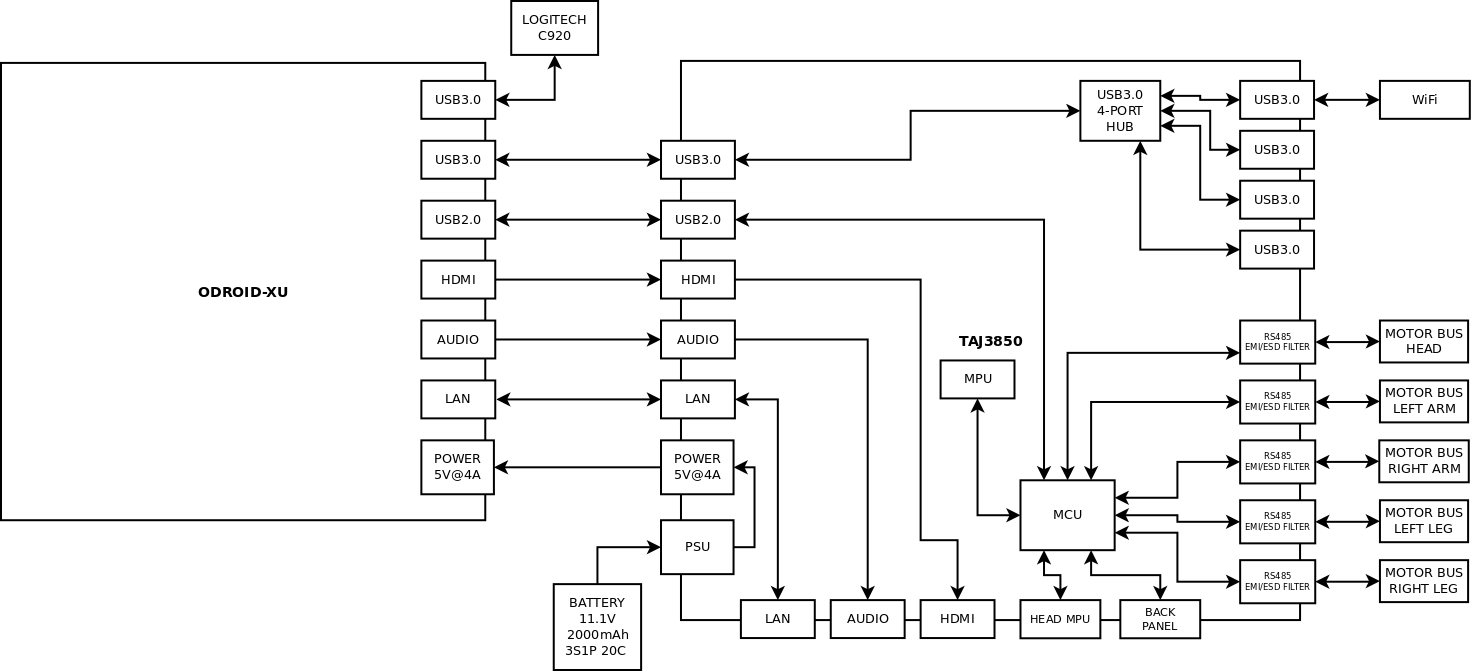
\includegraphics[angle=270]{TAJ3850.png}}
%\caption{Connection mappings between the TAJ3850, ODroid-XU, and external peripherals.}
%\label{fig:taj3850}
%\end{center}
%\end{figure}

%The above enhancements will not be implemented on all of the DARwIn-OP robots.


\subsection*{Acknowledgement} The NUbot team is greatful to their main industrial partners and sponsors 4Tel Pty. Ltd and Tribotix. They also would like to thank the School of Electrical Engineering and Computing, and the Faculty of Engineering and Built Environment at The University of Newcastle, Australia, for continued support. Alex Biddulph and Trent Houliston were supported by an Australian Government Research Training Program scholarship and a top-up scholarship through 4Tel~Pty.~Ltd.


\bibliographystyle{plain}
% argument is your BibTeX string definitions and bibliography database(s)
\bibliography{nubots}

\end{document}
